\documentclass[]{beamer}
\usepackage[T1]{fontenc}
\usepackage[utf8]{inputenc}
\usepackage{lmodern}
\usepackage[italian]{babel}

\title{Le reti e la sicurezza informatica}
\author{Mattia Cozzi\newline\href{mailto:cozzimattia@gmail.com}{\texttt{cozzimattia@gmail.com}}}
\date{a.s.~2023/2024}


%\documentclass[handout]{beamer}     %usare questa classe per generare l'handout

%\usepackage{pdfpages}   %per mostrare più quadri nella stessa pagina
%\pgfpagesuselayout{4 on 1}[a4paper,border shrink=5mm,landscape]


\usetheme{Singapore}
%\useoutertheme[left]{sidebar} %elementi intorno alle diapositive
\setbeamercovered{dynamic} %modifica l'aspetto del testo grigetto delle diapositive future. Argomenti: invisible/transparent/dynamic


%COLORE PRINCIPALE
\definecolor{verde}{RGB}{2, 194, 117} % UBC Blue (primary)
\setbeamercolor{structure}{fg=verde} % itemize, enumerate, etc
\setbeamercolor{alerted text}{fg=verde}


\usecolortheme{orchid}

\usepackage{tikz}

\begin{document}

\begin{frame}
  \titlepage
\end{frame}


\begin{frame}
\frametitle{Contenuti}
\tableofcontents
\end{frame}



\section{Classificazioni}


\begin{frame}
\frametitle{Collegamento}
I computer vengono collegati tra loro per:
\begin{itemize}
  \item comunicare tra loro;\pause
  \item condividere risorse:\pause
  \begin{itemize}
    \item hardware (stampanti);\pause
    \item files (su dischi fissi condivisi);\pause
    \item programmi o interi sistemi operativi;\pause
  \end{itemize}
\end{itemize}

~

Il collegamento avviene tramite un componente hardware chiamato \alert{scheda di rete}.
\end{frame}


\begin{frame}
\frametitle{Dimensione delle reti (1)}
Possiamo classificare le reti in base alla loro \alert<1>{dimensione}:\pause
\begin{description}
  \item[] Reti locali:
  \item[(W)LAN] ((Wireless) Local Area Network), terminali connessi nello stesso luogo (casa, ufficio);\pause
  \item[MAN] (Metropolitan Area Network), terminali in un'area urbana o comuni limitrofi;\pause
  \item[] Reti geografiche:
  \item[WAN] (Wide Area Network), terminali in un'intera nazione;\pause
  \item[GAN] (Global Area Network), terminali in tutti i continenti.
\end{description}\pause

~

Ogni terminale è identificato da un numero, l'indirizzo MAC (Media Access Control), univoco. Esempio di MAC:
\begin{center}
  \texttt{00-08-74-4C-7F-1D} (esadecimale)
\end{center}
\end{frame}


\begin{frame}
  \frametitle{Dimensione delle reti (2)}
\begin{figure}
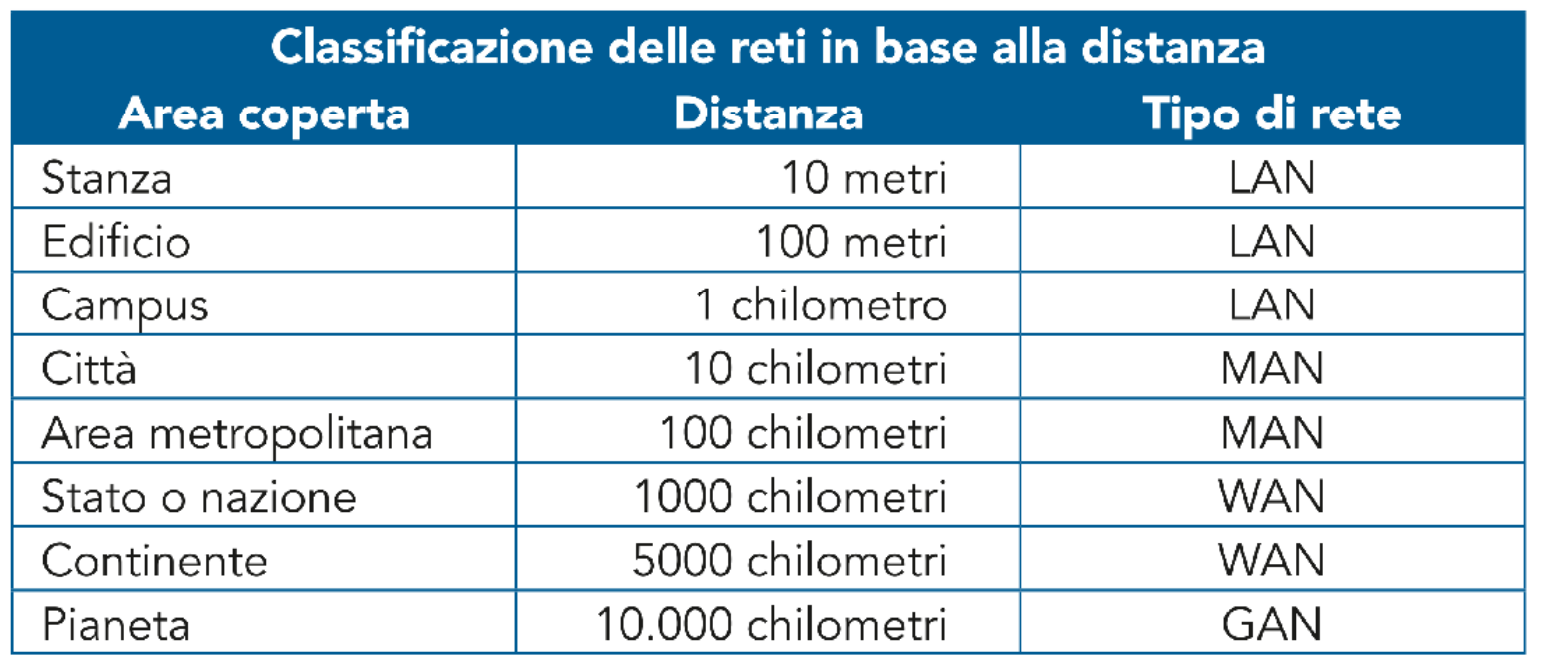
\includegraphics[width=.9\columnwidth]{img/dimensionereti.png}
\end{figure}
\end{frame}


\begin{frame}
\frametitle{Modello client/server e peer to peer}
Come avviene la condivisione di risorse?\pause

~

Dividiamo le reti in due classi:
\begin{description}
  \item[client/server] alcuni computer (server o host) mettono a disposizione risorse, altri (client) le utilizzano;\pause
  \item[peer to peer] tutti i computer condividono le loro risorse e tutti possono utilizzarle.\pause
\end{description}

~

Nel modello peer to peer ogni computer è sia server sia client.
\end{frame}

\begin{frame}
\frametitle{Schema del modello client-server}
\begin{figure}
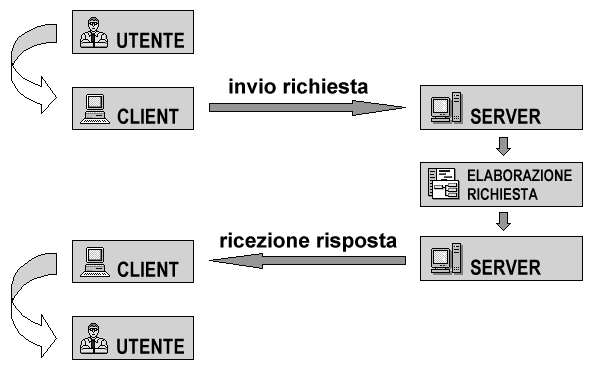
\includegraphics[width=.7\columnwidth]{screenshots/clientserver.png}
\end{figure}
\end{frame}

\begin{frame}
\frametitle{Topologia delle reti (1)}
Quando realizziamo una rete, possiamo darle una diversa struttura a seconda delle necessità che si hanno.\pause

~

\begin{itemize}
  \item A \alert<2->{maglia} (mesh), in cui tutti i nodi sono collegati a tutti gli altri nodi.
  
  ~

  \visible<2->{\begin{figure}
    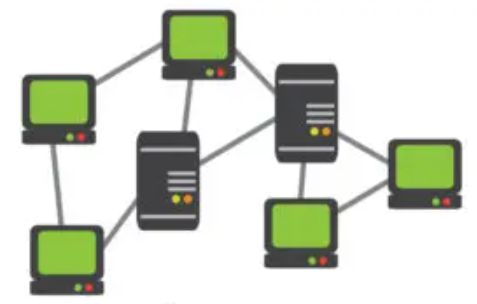
\includegraphics[width=.4\columnwidth]{img/maglia.png}
  \end{figure}}\pause 

  ~

  Garantisce alta tolleranza all'errore ed è molto veloce. Complessa da realizzare su larga scala.
\end{itemize}
\end{frame}

\begin{frame}
\frametitle{Topologia delle reti (2)}
  \begin{itemize}
    \item A \alert<1->{stella}, con un nodo principale al centro.
    
    ~

    \visible<1->{\begin{figure}
      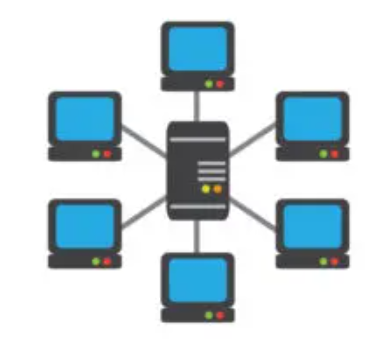
\includegraphics[width=.3\columnwidth]{img/stella.png}
    \end{figure}}\pause 

    ~

    Garantisce tolleranza all'errore ed è facile da espandere. Richiede un hub centrale affidabile.
  \end{itemize}
\end{frame}


\begin{frame}
\frametitle{Topologia delle reti (3)}
  \begin{itemize}
    \item Ad \alert<1->{anello}.
    
    ~

    \visible<1->{\begin{figure}
      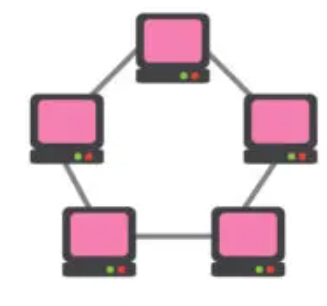
\includegraphics[width=.25\columnwidth]{img/anello.png}
    \end{figure}}\pause

    ~

    Garantisce semplicità di costruzione, ma ha bassa tolleranza ai guasti.
  \end{itemize}
\end{frame}


\begin{frame}
\frametitle{Topologia delle reti (4)}
  \begin{itemize}
    \item Ad \alert<1->{albero}, con un nodo radice (root) collegato ai nodi secondari (leaves).
    
    ~

    \visible<1->{\begin{figure}
      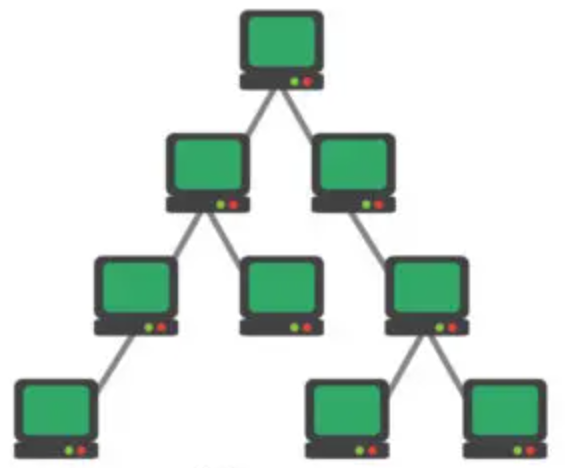
\includegraphics[width=.3\columnwidth]{img/albero2.png}
    \end{figure}}\pause

    ~

    Ha costi contenuti ed è facilmente espandibile, ma ha scarsissima tolleranza ai guasti.
  \end{itemize}
\end{frame}

\begin{frame}
\frametitle{Topologia delle reti (5)}
  \begin{itemize}
    \item A \alert<1->{bus}, con un cavo centrale detto ``dorsale'' o bus.
    
    ~

    \visible<1->{\begin{figure}
      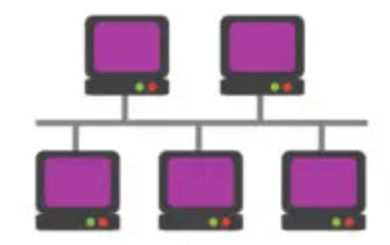
\includegraphics[width=.3\columnwidth]{img/bus.png}
    \end{figure}}\pause

    ~

    Costi bassi, facilmente espandibile. Scarsa tolleranza ai guasti e velocità che dipende solo dal cavo principale.
  \end{itemize}
\end{frame}


\begin{frame}
\frametitle{Tecnica di commutazione}
Come vengono trasmessi i dati in una rete?\pause

~

Esistono due modalità, una derivata dalla rete telefonica e una utilizzata nelle reti informatiche:
\begin{itemize}
  \item a \alert<2>{commutazione di circuito}, che prevede l'attivazione del circuito di comunicazione tra mittente e ricevente, invia i dati e chiude la comunicazione; in questo caso tutto il canale viene utilizzato per la comunicazione;\pause
  \item a \alert<3>{commutazione di pacchetto}, in cui i messaggi sono spezzati in segmenti e poi ricomposti a destinazione; uno stesso canale viene condiviso da più pacchetti per destinatari diversi.
\end{itemize}
\end{frame}


\begin{frame}
\frametitle{Packet switching}
Nella commutazione di pacchetto viene utilizzata la tecnica dell'\alert<1>{instradamento} ove non sono presenti collegamenti fisici diretti tra due apparecchi, ma logici.\pause

~

Un pacchetto presenta informazioni aggiuntive rispetto al dato puro: sono ad esempio definiti mittente e destinatario (imbustamento).\pause

~

Un pacchetto si divide in:
\begin{itemize}
  \item \alert<3>{header}: intestazione pacchetto con mittente e destinatario e numero progressivo (per ricomporre correttamente il messaggio a destinazione);\pause
  \item \alert<4>{payload}: i dati da trasmettere.
\end{itemize}
\end{frame}


\section{Networking}

\begin{frame}
\frametitle{Rete aziendale}
Una rete aziendale è una rete che serve a condividere le risorse informatiche di un'azienda (files e documenti, ma anche stampanti e altro).\pause

~

È necessaria la presenza di uno \alert<2>{switch}, un dispositivo che permette di smistare il traffico di dati sui vari terminali.\pause

~

Per collegare la rete aziendale all'esterno (come alla rete internet) è necessario un \alert<3>{router}. I dati sono protetti da un \alert<3>{firewall}.\pause

~

I dispositivi connessi devono possedere ovviamente una \alert<4>{scheda di rete}.
\end{frame}

\begin{frame}
\frametitle{VPN}
Spesso le aziende (e ultimamente anche i privati) utilizzano una VPN (Virtual Private Network).\pause

~

La VPN permette di inviare dati in maniera criptata (e quindi sicura) ad un server esterno, che si interfaccia poi con la rete internet.

\visible<2->{\begin{figure}
  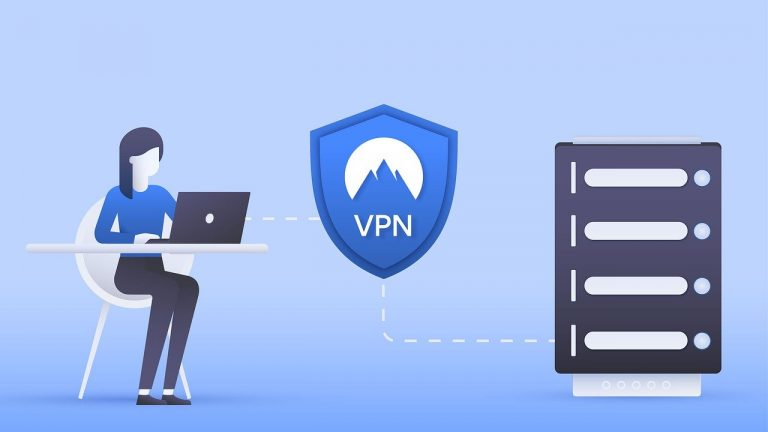
\includegraphics[width=.5\columnwidth]{img/vpn.jpg}
\end{figure}}
\end{frame}


\begin{frame}
\frametitle{Progettazione di una rete}
Quando si progetta o si configura una rete aziendale è bene immaginarsene la struttura sulla base delle \alert<1>{dimensioni} che la rete avrà e della distribuzione degli spazi.\pause

~

Ad influenzare le scelte sarà anche il modo con cui le informazioni sono archiviate, e da quale punto della rete dovranno essere rese accessibili, e ancora quali sono gli hardware e i sistemi di sicurezza a disposizione.
\end{frame}



\begin{frame}
\frametitle{Internet, Intranet, Extranet}
\begin{itemize}
  \item Una \alert<1->{internet} è una rete che, mediante il protocollo TCP/IP, permette di collegare tra loro più reti locali e/o reti geografiche. L’esempio più comune di rete internet è l’omonima rete informatica (Internet, con la i maiuscola).\pause
  
  ~

  \item Una \alert<2->{intranet} è una rete privata, spesso sotto forma di LAN. È accessibile solo ad una determinata cerchia di utenti. Una intranet può essere isolata da Internet oppure esservi connessa. Un esempio sono le reti casalinghe.\pause
  
  ~

  \item Una \alert<3>{extranet} è una rete informatica che permette anche a soggetti esterni alla LAN di accedere a informazioni e dati. È una rete privata controllata da un'organizzazione che ne consente l’accesso solo a determinati utenti autorizzati.
\end{itemize}
\end{frame}



\begin{frame}
\frametitle{Protocolli}
Le reti sono organizzate a \alert<1>{livelli} standardizzati per facilitare la comunicazione.\pause

~

Si ha una \alert<2>{struttura gerarchica} per cui ogni livello può comunicare solo con il superiore e con l’inferiore, mediante diverse interfacce.\pause

~

Gli standard per la comunicazione sono detti \alert<3>{protocolli}.
\end{frame}


\begin{frame}
\frametitle{Modello ISO-OSI (1)}
Lo standard \emph{teorico} è il modello ISO/OSI (1984), su \alert<1->{sette livelli}:\pause
\begin{columns}
\begin{column}{.55\textwidth}
  \begin{enumerate}
    \item \alert<2>{applicazione}: fornisce i protocolli utilizzati dalle specifiche applicazioni;\pause
    \item \alert<3>{presentazione}: permette di gestire la sintassi dei messaggi, convertendo tra protocolli;\pause
    \item \alert<4>{sessione}: controlla la connessione tra applicazioni cooperanti e sincronizza tra invio e ricezione;
  \end{enumerate}
\end{column}
\begin{column}{.45\textwidth}
  \visible<1->{\begin{figure}
    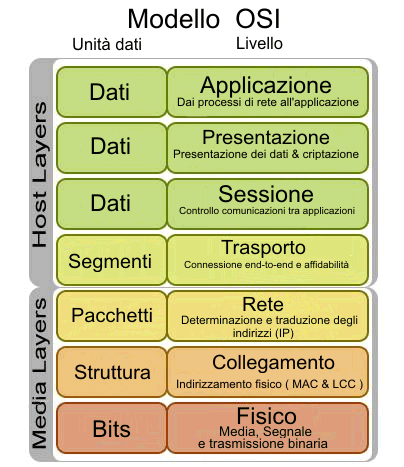
\includegraphics[width=\columnwidth]{img/isoosi.png}
  \end{figure}}
\end{column}
\end{columns}
\end{frame}



\begin{frame}
\frametitle{Modello ISO-OSI (2)}
\begin{columns}
\begin{column}{.55\textwidth}
  \begin{enumerate}\setcounter{enumi}{3}
    \item \alert<1>{trasporto}: stabilisce e mantiene la connessione, controlla la congestione e gli errori;\pause
    \item \alert<2>{rete}: si occupa del routing, la scelta del percorso ottimale nella rete per il messaggio;\pause
    \item \alert<3>{collegamento}: controlla il flusso di dati e gli errori, se necessario richiede i dati errati;\pause
    \item \alert<4>{fisico}: si occupa dell’hardware, delle tensioni e durate dei segnali su cavo o via onde elettromagnetiche.
  \end{enumerate}
\end{column}
\begin{column}{.45\textwidth}
  \begin{figure}
    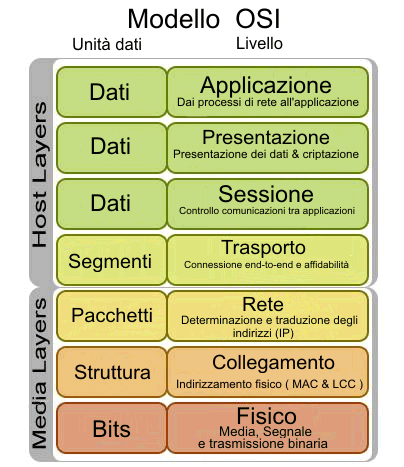
\includegraphics[width=\columnwidth]{img/isoosi.png}
  \end{figure}
\end{column}
\end{columns}
\end{frame}

\begin{frame}
\frametitle{Protocollo TCP-IP}
Il modello ISO-OSI è piuttosto complesso e di fatto viene utilizzato il più semplice TCP-IP.\pause

~

L’acronimo significa \alert<2>{Transfer Control Protocol/Internet Protocol}.\pause

~


È composto di soli quattro livelli:
\begin{columns}
\begin{column}{.3\textwidth}
  \begin{enumerate}
    \item \alert<3>{applicazione} (es.~browser);\pause
    \item \alert<4>{TCP/UDP};\pause
    \item \alert<5>{IP};\pause
    \item \alert<6>{Ethernet}.
  \end{enumerate}
\end{column}
\begin{column}{.5\textwidth}
  \visible<3->{\begin{figure}
    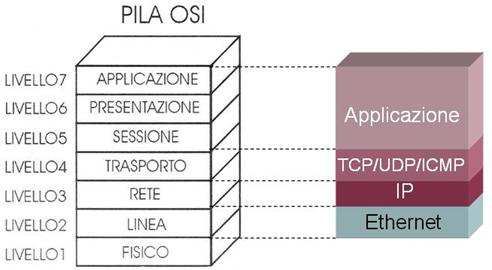
\includegraphics[width=\columnwidth]{img/tcpip.png}
  \end{figure}}
\end{column}
\end{columns}
\end{frame}



\begin{frame}
\frametitle{Indirizzi IP}
L'indirizzo IP è composto da \alert<1>{4 cifre da 0 a 255 separate da punti} e serve a identificare in modo univoco un dispositivo in rete.\pause

~

Ogni numero è a 8 bit, quindi dato in numerazione binaria con 8 cifre che possono essere 0 o 1. In totale abbiamo \alert<2>{32 bit}.\pause

~

\visible<3->{\begin{figure}
  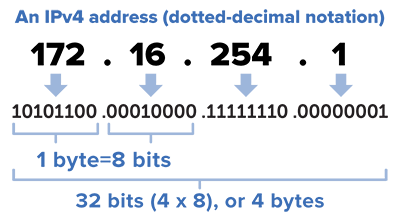
\includegraphics[width=.6\columnwidth]{img/ip.png}
\end{figure}}
  

\end{frame}



\section{Internet}


\begin{frame}
\frametitle{Storia}
\begin{description}
  \item[1969] Il progetto ARPANET, finanziato dal Dipartimento della Difesa statunitense è la prima rete mai costruita, ottenuta collegando quattro nodi. Le applicazioni eseguite erano principalmente programmi di File Transfer Protocol (FTP).\pause
  \item[1971] Viene inventata la posta elettronica. I nodi salgono a 15, con 23 hosts.\pause
  \item[1973] Viene sviluppato il protocollo TCP/IP.\pause
  \item[1991] Tim Berners-Lee inventa il protocollo HTTP e il linguaggio HTML: nasce la rete internet moderna.\pause
  \item[1993] Nasce il primo browser, Mosaic.
\end{description}
\end{frame}

\begin{frame}
\frametitle{La prima rete}
\begin{figure}
    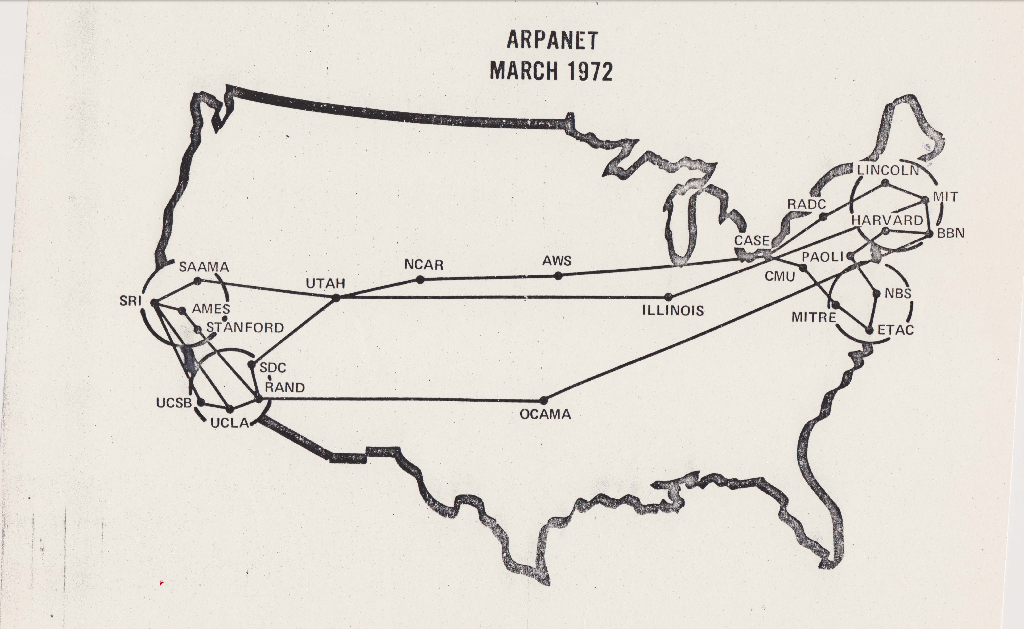
\includegraphics[width=.9\columnwidth]{img/arpanet.png}
  \end{figure}
\end{frame}


\begin{frame}
\frametitle{Una rete globale distribuita}
Un aspetto importante di Internet è la sua \alert<1>{topologia distribuita e decentrata}: è formata dall'integrazione di numerose sottoreti pubbliche, commerciali e private.\pause

~

Se un percorso è interrotto o troppo trafficato i dati possono prendere strade alternative.

~

\begin{figure}
  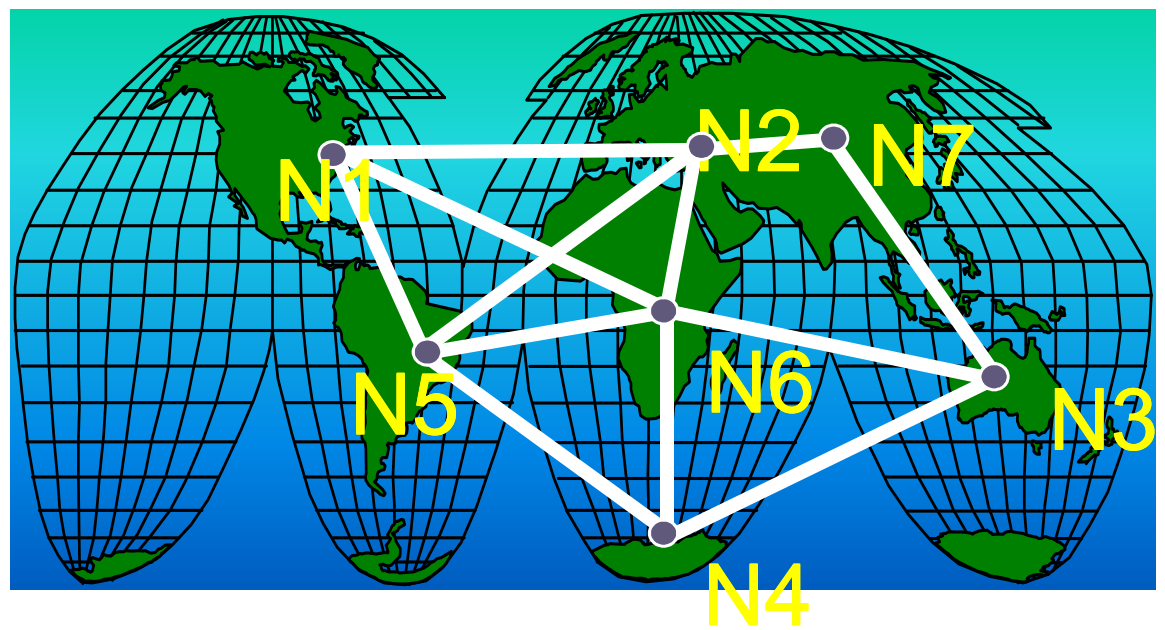
\includegraphics[width=.5\columnwidth]{img/percorsi.png}
\end{figure}
\end{frame}


\begin{frame}
\frametitle{Il web}
Il \alert<1->{World Wide Web} (WWW) è il principale servizio di internet: è l'insieme dei documenti (pagine web o altro) collegati tra loro.\pause

~

Il collegamento avviene mediante \alert<2>{hyperlinks} (o links, o collegamenti ipertestuali).\pause

~

Le pagine web sono particolari tipi di documenti chiamati \alert<3>{ipertesti} e sono scritte in linguaggio HTML (HyperText Markup Language).
\end{frame}


\begin{frame}
\frametitle{Indirizzi}
Ogni risorsa è identificata da un \alert<1>{indirizzo} (URL, uniform resource locator). Un semplice esempio:\pause

\begin{center}
  \visible<2->{\alert<2>{\texttt{https://}}}\visible<3->{\alert<3>{\texttt{www.}}}\visible<4->{\alert<4>{\texttt{google}}}\visible<5->{\alert<5>{\texttt{.it}}}
\end{center}

~

Un indirizzo contiene:
\begin{itemize}
  \item un \alert<2>{protocollo} (come \texttt{http} o \texttt{https}, più sicuro);\pause
  \item l'indicazione del \alert<3>{servizio} (come \texttt{www} per il web);\pause
  \item un \alert<4>{dominio di secondo livello} (cioè il nome della risorsa, sito);\pause
  \item un \alert<5>{dominio di primo livello} (come \texttt{.it} o \texttt{.com}).\pause
\end{itemize}

~

Gli URL sono in realtà costituti da indirizzi IP, associati ad un testo da un DNS (Domain Name System).
\end{frame}


\begin{frame}
\frametitle{Navigare in rete: il browser}
Per visualizzare le risorse presenti online (come i siti web) è necessario un \alert<1>{browser} (letteralmente ``sfogliatore''), che permette di \alert<1>{navigare in internet}.

~

\begin{figure}
  
\includegraphics[width=.7\columnwidth]{img/browsers.png}
\end{figure}\pause

~

Quando visualizziamo una pagina, l'utente digita un URL, il browser la richiede al server. Se il server risponde positivamente, fornisce la risorsa al browser, che la mostra all'utente.
\end{frame}

% \begin{frame}
% \frametitle{Navigare in rete}

% https://bertola.eu/usenet/faq/testi/icfaq-demo/fondamen.htm

% \end{frame}


\begin{frame}
\frametitle{Il linguaggio HTML}
Il linguaggio HTML è un \alert<1>{linguaggio di marcatori} che permette di scrivere le pagine web.\pause

~

È costituito da testo semplice con specifici codici che vengono \alert<2>{interpretati graficamente} dal browser.

\begin{columns}
  \begin{column}{0.45\textwidth}
  \begin{figure}
  \visible<2>{\fbox{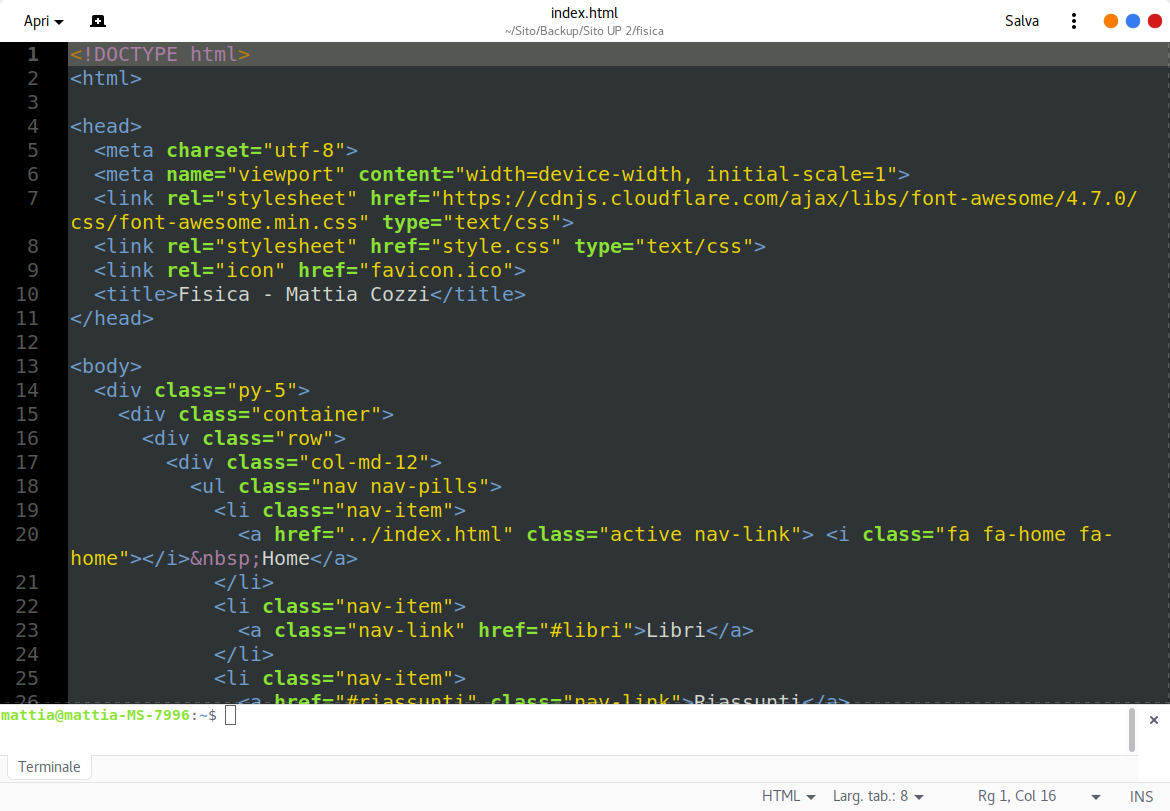
\includegraphics[width=\columnwidth]{screenshots/sitotesto.png}}
  
  Testo semplice}
  \end{figure}
  \end{column}
  \begin{column}{0.45\textwidth}
  \begin{figure}
  \visible<2>{\fbox{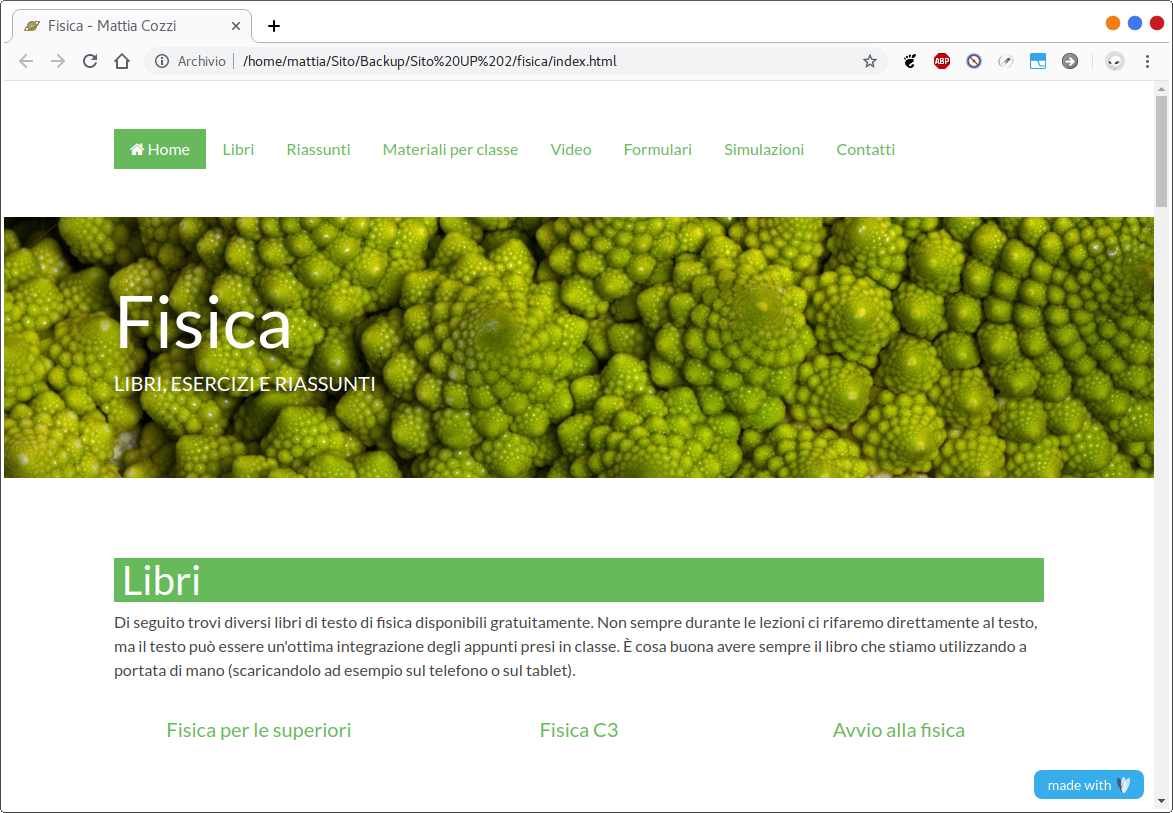
\includegraphics[width=\columnwidth,]{screenshots/sitoformattato.png}}
  
  Pagina visualizzata}
  \end{figure}
  \end{column}
\end{columns}
\end{frame}



\begin{frame}
\frametitle{Motori di ricerca}
Un motore di ricerca è un sito che permette di fornire un \alert<1>{elenco di pagine} che contengono informazioni che l'utente richiede.\pause

~

Le pagine sono selezionate tramite le \alert<2>{parole chiave} inserite dall'utente nella \alert<2>{casella di ricerca}.\pause

~

L'ordine con cui le pagine vengono visualizzate è stabilito da un algoritmo chiamato \alert<3>{ranking}.
\end{frame}



\begin{frame}
\frametitle{Ricerca avanzata}
Google, il motore di ricerca più utilizzato attualmente, contiene molte funzioni di ricerca avanzate:\pause
\begin{itemize}
  \item ricerca di stringa esatta, con \texttt{"nel mezzo del cammin"};\pause
  \item ricerca tramite \emph{wildcard}, cioè l'asterisco, con \texttt{nel * del cammin};\pause
  \item ricerca di pagine che non contengono una certa parola, con \texttt{-dante};\pause
  \item calcoli matematici e conversioni, da inserire direttamente nella barra di ricerca;\pause
  \item selezionare pagine pubblicate in date specifiche, scritte in una certa lingua, ecc.;\pause
  \item trovare immagini con specifiche caratteristiche di colore, dimensione, proporzioni, stile. 
\end{itemize}
\end{frame}


\begin{frame}
\frametitle{Esempio}
\begin{columns}
\begin{column}{.5\textwidth}
  \begin{figure}
    Ricerca:\\\texttt{Italia}

    ~

    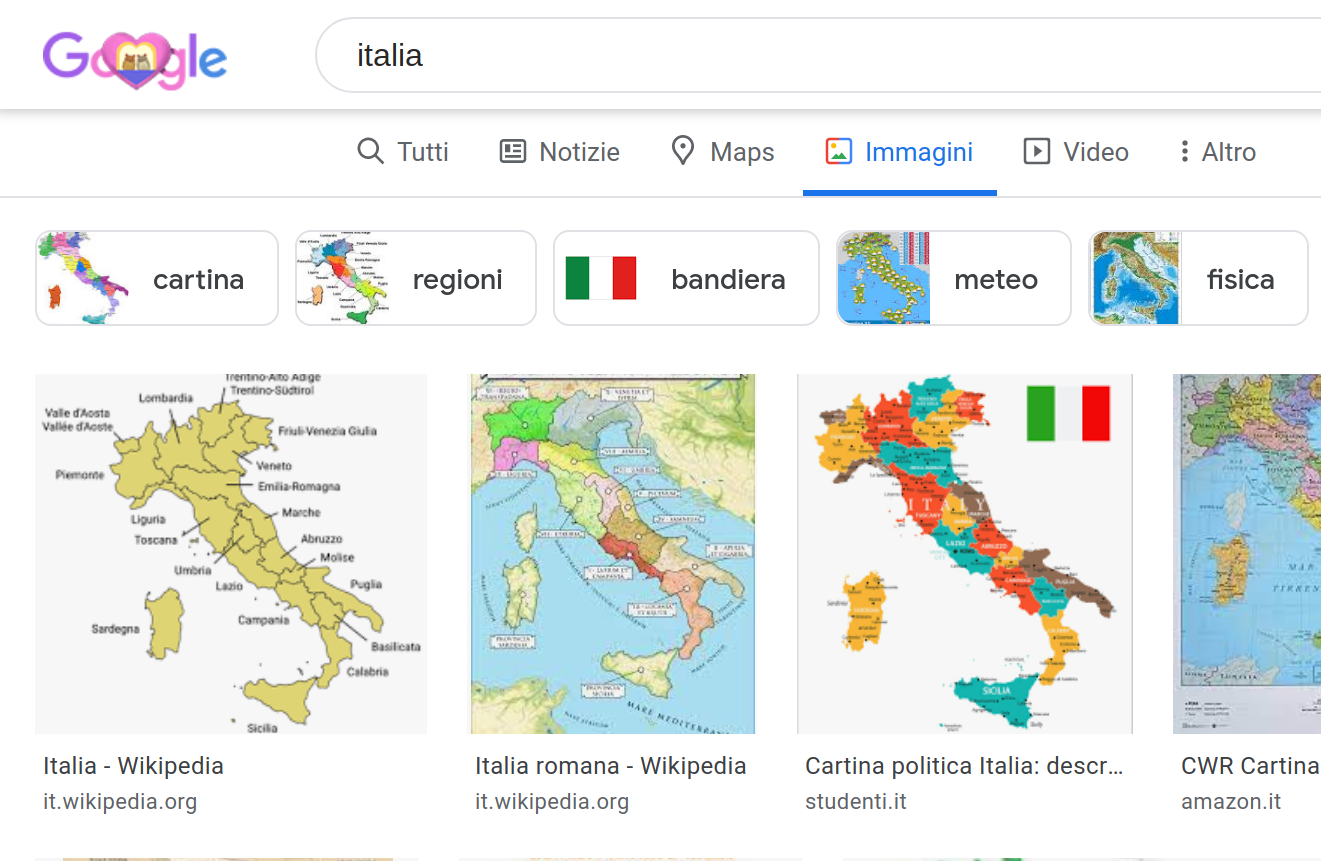
\includegraphics[width=\columnwidth]{img/italia.png}
  \end{figure}
\end{column}
\begin{column}{.5\textwidth}
  \begin{figure}
    Ricerca:\\\texttt{Italia -mappa}
    
    ~

    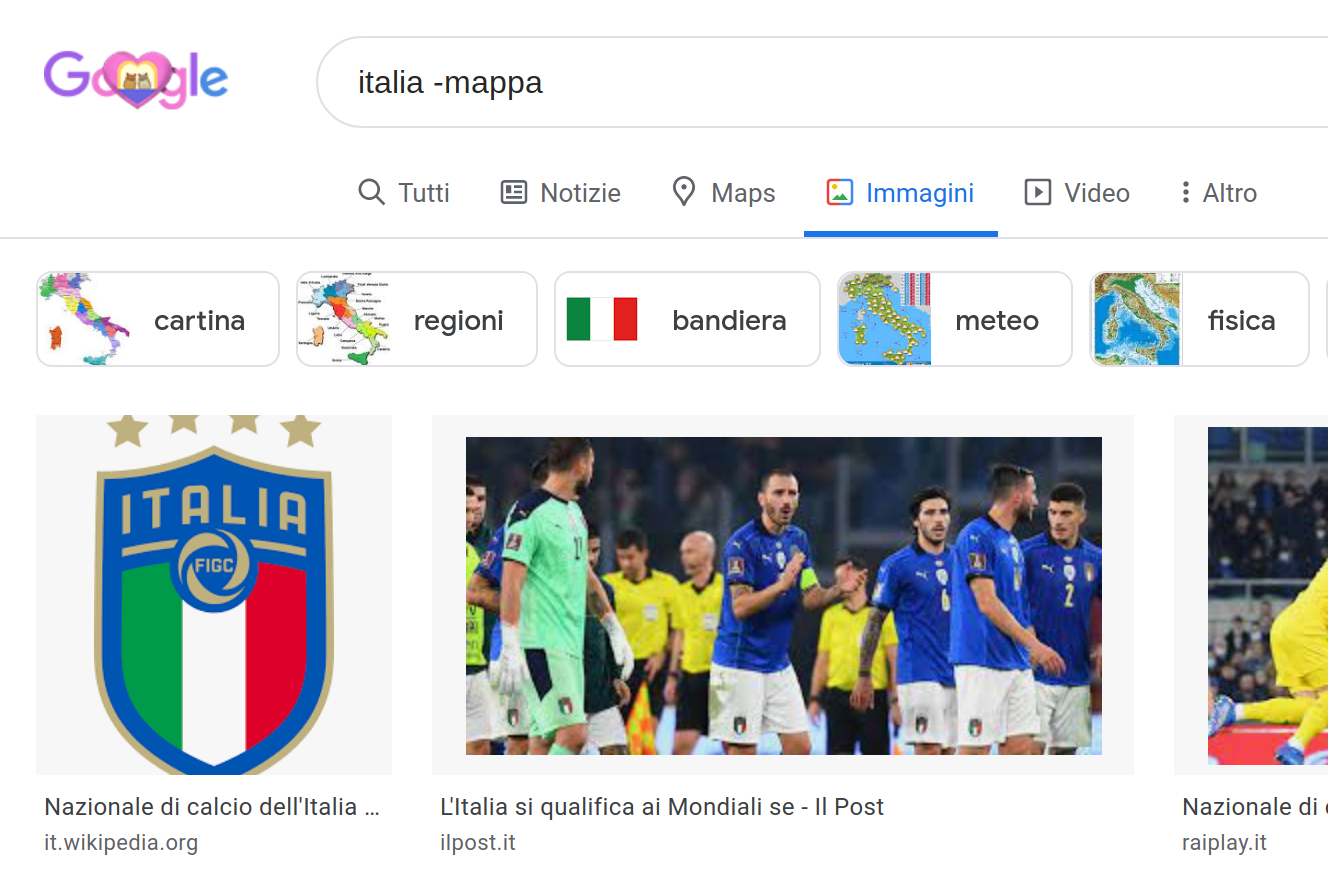
\includegraphics[width=\columnwidth]{img/italia2.png}
  \end{figure}
\end{column}
\end{columns}
\end{frame}


\begin{frame}
\frametitle{Valutazione critica delle informazioni}
L'enorme quantità di informazioni disponibili sul Web (pubblicabili da qualunque utente della rete) rende necessaria una loro \alert<1>{valutazione critica}.\pause

~

Dobbiamo sempre considerare la \alert<2>{credibilità} di un sito/video, ecc. Fattori importanti possono essere ad esempio le fonti citate da una notizia.\pause

~

Il Web, rispetto alla carta stampata, può essere più insidioso, perché manca quasi completamente il controllo editoriale della correttezza delle informazioni.
\end{frame}


\begin{frame}
\frametitle{La posta elettronica}
La posta elettronica (\alert<1>{email}) è la modalità di comunicazione più importante offerta da internet.\pause

~

\begin{columns}
  \begin{column}{0.55\textwidth}
  Un indirizzo email è costituito da un nome utente (\texttt{cozzimattia}), dal simbolo $@$ (si legge ``at'') e da un dominio (\texttt{gmail.com}).\pause

   ~
   
   Ogni email possiede un \alert<3>{oggetto} (l'argomento del messaggio), un \alert<3>{testo/contenuto} ed eventualmente uno o più \alert<3>{allegati}.
  \end{column}
  \begin{column}{0.37\textwidth}
  \visible<3>{\begin{figure}
  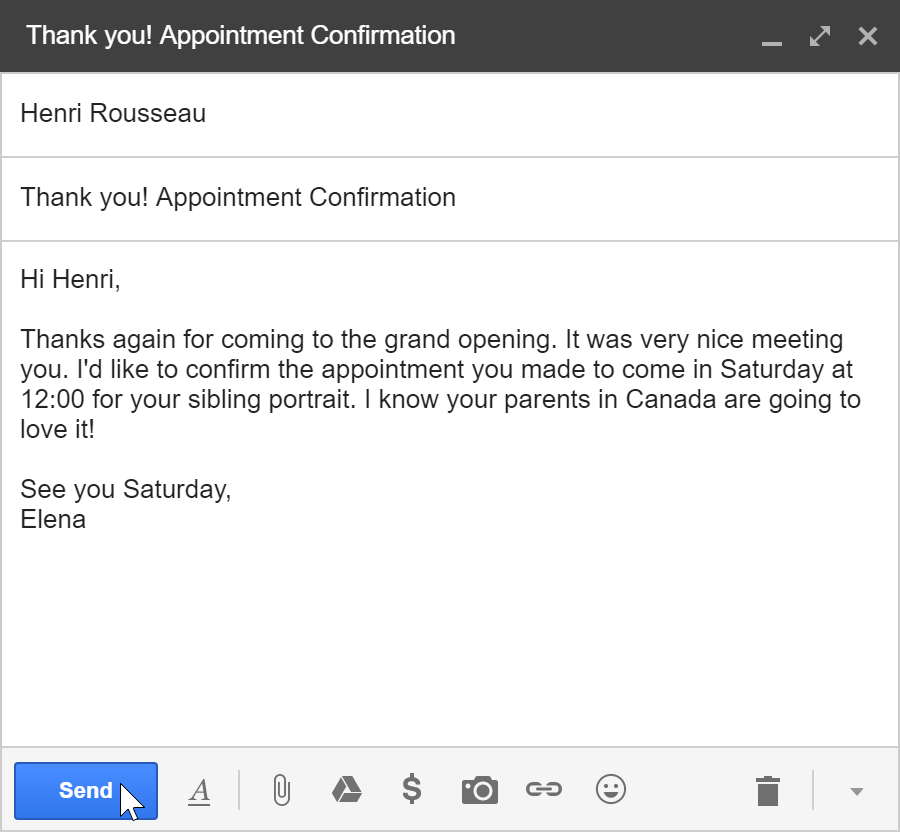
\includegraphics[width=\columnwidth]{img/email.png}
  \end{figure}}
  \end{column}
\end{columns}
\end{frame}



\begin{frame}
\frametitle{Campi per i destinatari}
Esistono tre categorie di destinatari per un messaggio email:
\begin{columns}
  \begin{column}{0.5\textwidth}
  \begin{itemize}
   \item \alert<1>{A}, per uno o più destinatari principali;\pause
   \item \alert<2>{Cc} (copia per conoscenza), per destinatari secondari;\pause
   \item \alert<3>{Ccn} (copia conoscenza nascosta), per destinatari che però non possono sapere a quali altri indirizzi (in Cc) la mail è stata inviata.
  \end{itemize}
  \end{column}
  \begin{column}{0.4\textwidth}
  \begin{figure}
  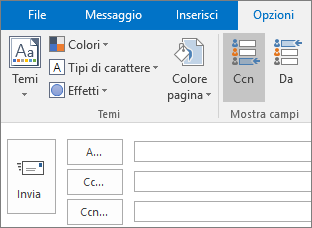
\includegraphics[width=\columnwidth]{img/accccn.png}
  \end{figure}
  \end{column}
\end{columns}
\end{frame}



\begin{frame}
\frametitle{Poter accedere}
È fondamentale, per poter usare la maggior parte dei servizi online, possedere un \alert{account di posta elettronica}: viene sempre chiesto durante la registrazione a qualsiasi servizio.\pause

~

Dobbiamo quindi \alert{sempre ricordare il nostro indirizzo email e la password per accedervi}.

\begin{figure}
  \frame{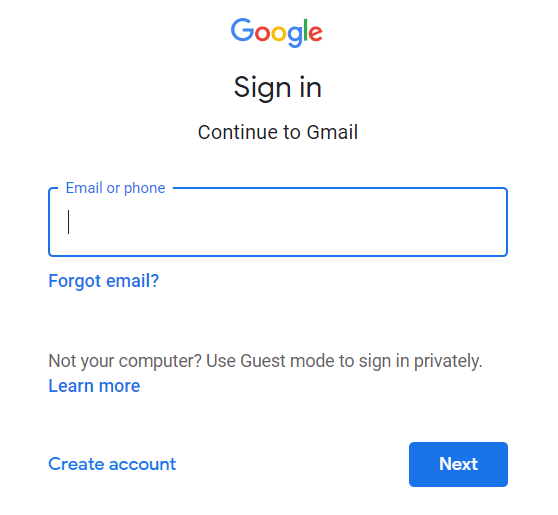
\includegraphics[width=.35\columnwidth]{img/signin.png}}
\end{figure}
\end{frame}

\begin{frame}
\frametitle{Forum}
Sul Web esistono numerosissimi forum, \alert<1>{piazze virtuali} in cui gli utenti discutono degli argomenti più disparati oppure chiedono consiglio ad utenti più esperti.\pause

~

Alcuni dei termini utilizzati sono:
\begin{itemize}
  \item \alert<2>{thread}, discussione, come in ``aprire un thread'';\pause
  \item \alert<3>{topic}, cioè l'argomento del thread; ``off-topic'' significa ``fuori tema'';\pause
  \item \alert<4>{mod}, cioè i moderatori del forum, che controllano che gli utenti rispettino le regole del forum;\pause
  \item \alert<5>{ban}, cioè l'espulsione (temporanea o definitiva) di un utente dal forum.
\end{itemize}
\end{frame}


\begin{frame}
\frametitle{Social media}
Internet è sempre stata usata per ``collegare le persone'': con email, chat oppure forum.\pause

~

Tuttavia i forum (siti web su cui è possibile postare messaggi e ricevere risposte da altri utenti) sono solitamente dedicati alla discussione su un argomento specifico.\pause

~

I social network ruotano invece (parzialmente) intorno alle informazioni sull'utente, oltre a veicolare contenuti pubblicitari.
\end{frame}



\begin{frame}
\frametitle{Netiquette}
Parlare con una persona online (ad esempio via email, su un blog o un social network) è un po' come parlare con una persona davanti a noi: ci sono delle \alert<1>{buone pratiche} di rispetto reciproco da mettere in atto.\pause

~

L'insieme di queste pratiche si chiama \alert<2->{netiquette}:\pause
\begin{itemize}
  \item chiedere il permesso di diffondere contenuti che coinvolgono altre persone;\pause
  \item evitare il bullismo digitale, in ogni sua forma;\pause
  \item cercare di esprimersi il più chiaramente possibile (scrivendo, ci si può fermare a pensare cosa scrivere);\pause
  \item evitare di scrivere sempre MAIUSCOLO (equivale ad urlare);\pause
  \item ecc.
\end{itemize}
\end{frame}


\section{Sicurezza}


\begin{frame}
\frametitle{Crittografia}
Le reti, per la loro natura condivisa, non sono mai perfettamente sicure. Trasferire dati sensibili (ad esempio i nostri estremi bancari) in rete può comportare dei rischi.\pause

~

La \alert<2>{crittografia} si occupa di garantire la riservatezza dei dati, l'affidabilità dei dati e che le autenticazioni siano veritiere.\pause

~

``Crittografia'' significa ``scrittura nascosta'' ed è il processo di codifica di un messaggio, in modo da renderlo illeggibile a persone non autorizzate.\pause

~

La codifica e la decodifica dei messaggi sono ottenute mediante \alert{algoritmi di cifratura}.
\end{frame}



\begin{frame}
\frametitle{Autenticazione}
\begin{columns}
\begin{column}{.6\textwidth}
  L'autenticazione è il servizio di sicurezza che permette di garantire l’identità degli interlocutori (utenti umani o computer).\pause

  ~

  ~

  ~

  L'autenticazione si può basare su:
\end{column}
\begin{column}{.3\textwidth}
  \begin{figure}
    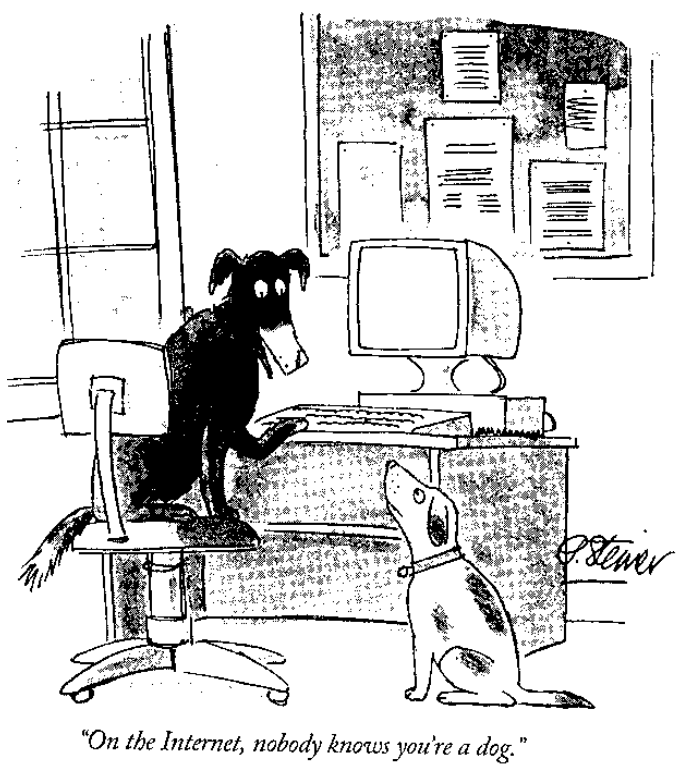
\includegraphics[width=\columnwidth]{img/dog.png}
  \end{figure}
\end{column}
\end{columns}
\begin{itemize}
  \item conoscenza di ``segreti'' (PIN, password);\pause
  \item possesso di cose fisiche o elettroniche (carte, token);\pause
  \item caratteristiche biometriche (volto, voce).\pause
\end{itemize}

~

Questi fattori si possono anche combinare tra loro.
\end{frame}



\begin{frame}
\frametitle{Username e password}
Il metodo di autenticazione più semplice è quello basato su username (nome che identifica l'utente) e password.\pause

~


Vantaggi:
\begin{itemize}
  \item semplice per l’utente;
  \item economico;
  \item non richiede di immagazzinare un segreto lato client.
\end{itemize}\pause

~

Svantaggi:
\begin{itemize}
  \item spesso gli utenti scelgono password deboli;
  \item spesso i metodi di autenticazione basati su password sono deboli.
\end{itemize}
\end{frame}




\begin{frame}
\frametitle{Antivirus}
Una delle attività più importanti per la sicurezza informatica è \alert<1>{installare un antivirus}.\pause

~

Un antivirus monitora continuamente le attività del computer, per identificarne di sospette ed eliminare le minacce note.\pause

~

Un antivirus ha accesso ad un database di virus e programmi malevoli, in modo da poterne individuare copie sul computer.\pause

~

I virus informatici cambiano continuamente, e quindi l'antivirus deve essere \alert<4>{costantemente aggiornato}.
\end{frame}



\begin{frame}
\frametitle{Malware}
La parola ``malware'' indica tutto l'insieme dei programmi dannosi per i computer.{\pause}

~

Possono essere:
\begin{itemize}
   \item \alert<2>{virus}, programmi che si autoreplicano all'interno di altri programmi o in qualche sezione del disco rigido;\pause
   \item \alert<3>{worm}, che si autoinviano a tutta la lista dei contatti e si diffondono principalmente mediante allegati email;\pause
   \item \alert<4>{trojan}, programmi dannosi nascosti all'interno di programmi innocui, che però non si possono autoreplicare;\pause
   \item \alert<5>{spyware}, programmi che una volta installati registrano e inviano le informazioni che passano nel sistema.
\end{itemize}
\end{frame}



\begin{frame}
\frametitle{Hacking}
L'hacking è spesso collegato ad attività criminose o comunque illecite. \pause

~

Nella sua definizione pià generale in realtà esso indica un processo per cui si fa uso della propria immaginazione e creatività per risolvere un problema complesso, con lo scopo di accrescere la conoscenza.\pause

~

Questo comporta l'acquisizione di una profonda conoscenza del sistema informatico su cui si opera, in modo non necessariamente criminoso.\pause

~

L'\alert{hacking etico} consiste nell'attività di studio, modifica, miglioria e creazione di sistemi informatici, per semplice curiosità o per lavoro.
\end{frame}


\begin{frame}
\frametitle{Firewall}
Il firewall (letteralmente ``parafuoco'') è un sistema di sicurezza che \alert<1>{filtra tutte le informazioni in ingresso e in uscita da una rete}.\pause

~

Un firewall è fondamentale per una rete aziendale o privata: un'eventuale intrusione nella rete comporterebbe la possibilità che vengano rubati dei dati.\pause

~

Un firewall può essere hardware (è un componente di una rete aziendale) e/o software, con specifici programmi installati sulle macchine connesse in rete.
\end{frame}




\begin{frame}
\frametitle{Cookies}
Il protocollo HTTP non permette che il server contattato ``riconosca'' un utente che si è già collegato per ricevere una risorsa.\pause

~

Le informazioni di accesso ai server sono quindi memorizzate nel browser, all'interno di files detti \alert<2>{cookies}.\pause

~

I cookies memorizzano la lingua che preferiamo usare e altri parametri, oltre ad essere usati per ricerche di mercato e pubblicità mirate in base all'utente.
\end{frame}



\begin{frame}
\frametitle{Spam}
Con la parola ``spam'' si indica l’\alert<1>{invio di messaggi di posta elettronica indesiderati}, di email sgradite, o non richieste, generalmente spedite con fini promozionali e commerciali da utenti spesso sconosciuti. Sinonimo è ``junk mail'', cioè ``posta spazzatura''.\pause

~

Oggi lo spam viene veicolato attraverso diversi canali: posta elettronica, ma anche chat, social network e altri servizi online.\pause

~

Se le mail indesiderate sono inviate da organizzazioni legali, è sempre presente in fondo alle mail un \alert<3>{link per disiscriversi}.
\visible<3>{\begin{figure}
  
\includegraphics[width=.7\columnwidth]{img/spam.png}
\end{figure}}
\end{frame}



\begin{frame}
\frametitle{Phishing}
Il \alert<1>{phishing} è una forma di spam che punta a indurre l'utente a \alert<1>{rivelare informazioni personali o riservate}.\pause

~
  
Si realizza inviando agli utenti mail molto somiglianti a vere mail da parte di organizzazioni o aziende (banche, poste, servizi di consegna pacchi, ecc.).\pause

~

In queste mail l'utente viene invitato a fornire la sua password o altri dati, eventualmente anche con link a siti fasulli.\pause

~

Alcune di queste mail vengono automaticamente filtrate dai server, ma è sempre bene controllare la veridicità di una mail (controllando ad esempio l'indirizzo da cui proviene).
\end{frame}

\begin{frame}
\frametitle{Esempio di phishing}
\begin{figure}
  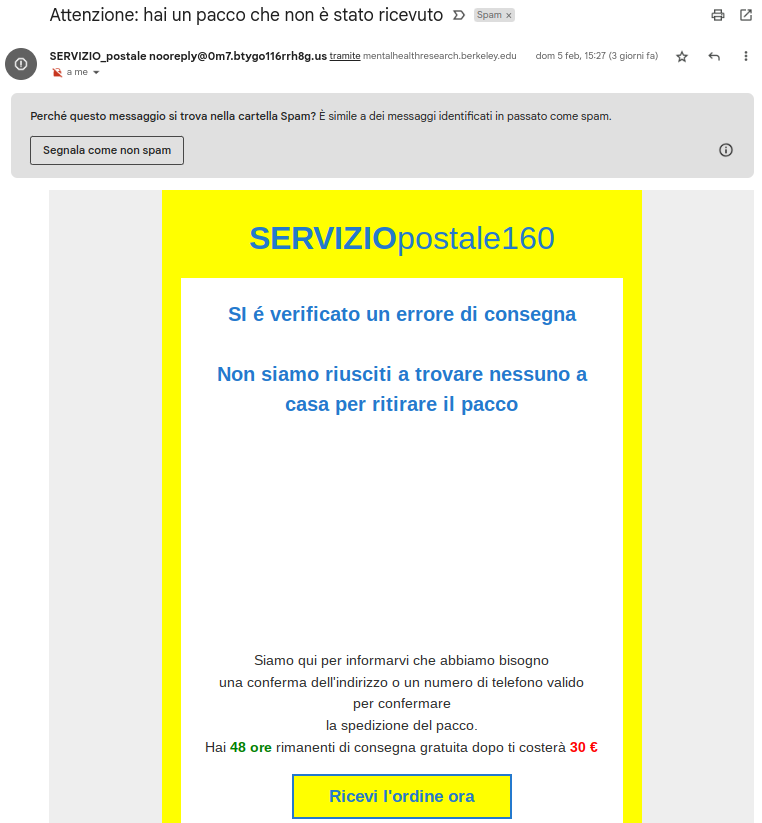
\includegraphics[width=.6\columnwidth]{img/phishing.png}
\end{figure}
\end{frame}



\begin{frame}
\frametitle{Firma elettronica e digitale}
I termini ``firma elettronica'' e ``firma digitale'' non sono equivalenti.\pause

~

La firma elettronica è un metodo di autenticazione che consente di associare dati ad altri dati, ed è un'espressione priva di valenza giuridica. I metodi per la firma elettronica sono stati descritti nella slide \alert<2>{Autenticazione}.\pause

~

La firma digitale è l'equivalente informatico di una tradizionale firma autografa e ha le caratteristiche di:
\begin{itemize}
  \item autenticità (garantisce l'identità del sottoscrittore);
  \item integrità (il documento non è stato modificato);
  \item non ripudio (ha valore giuridico e può essere usata nella PA).
\end{itemize}
\end{frame}



\begin{frame}
\frametitle{PEC}
La Posta Elettronica Certificata è un sistema di comunicazione simile all'email, con alcune caratteristiche di \alert<1>{sicurezza e certificazione} che rendono i messaggi ``garantiti''.\pause

~

Un documento inviato via PEC ha lo stesso valore legale di una raccomandata, come definito nel DPR 11 febbraio 2005 n.~68.\pause

~

Ogni impresa deve possedere un indirizzo PEC univoco iscritto nel Registro delle imprese, pena l'esclusione da detto Registro.\pause

~

La certificazione della PEC viene effettuata da appositi enti inclusi nell'{Elenco Pubblico dei Gestori accreditati}.
\end{frame}








\end{document}
